% !TEX root = paper.tex

\section {Results}
\label{sec:results}

\begin{figure}[!hbt]
	\centering
	\subfigure{ 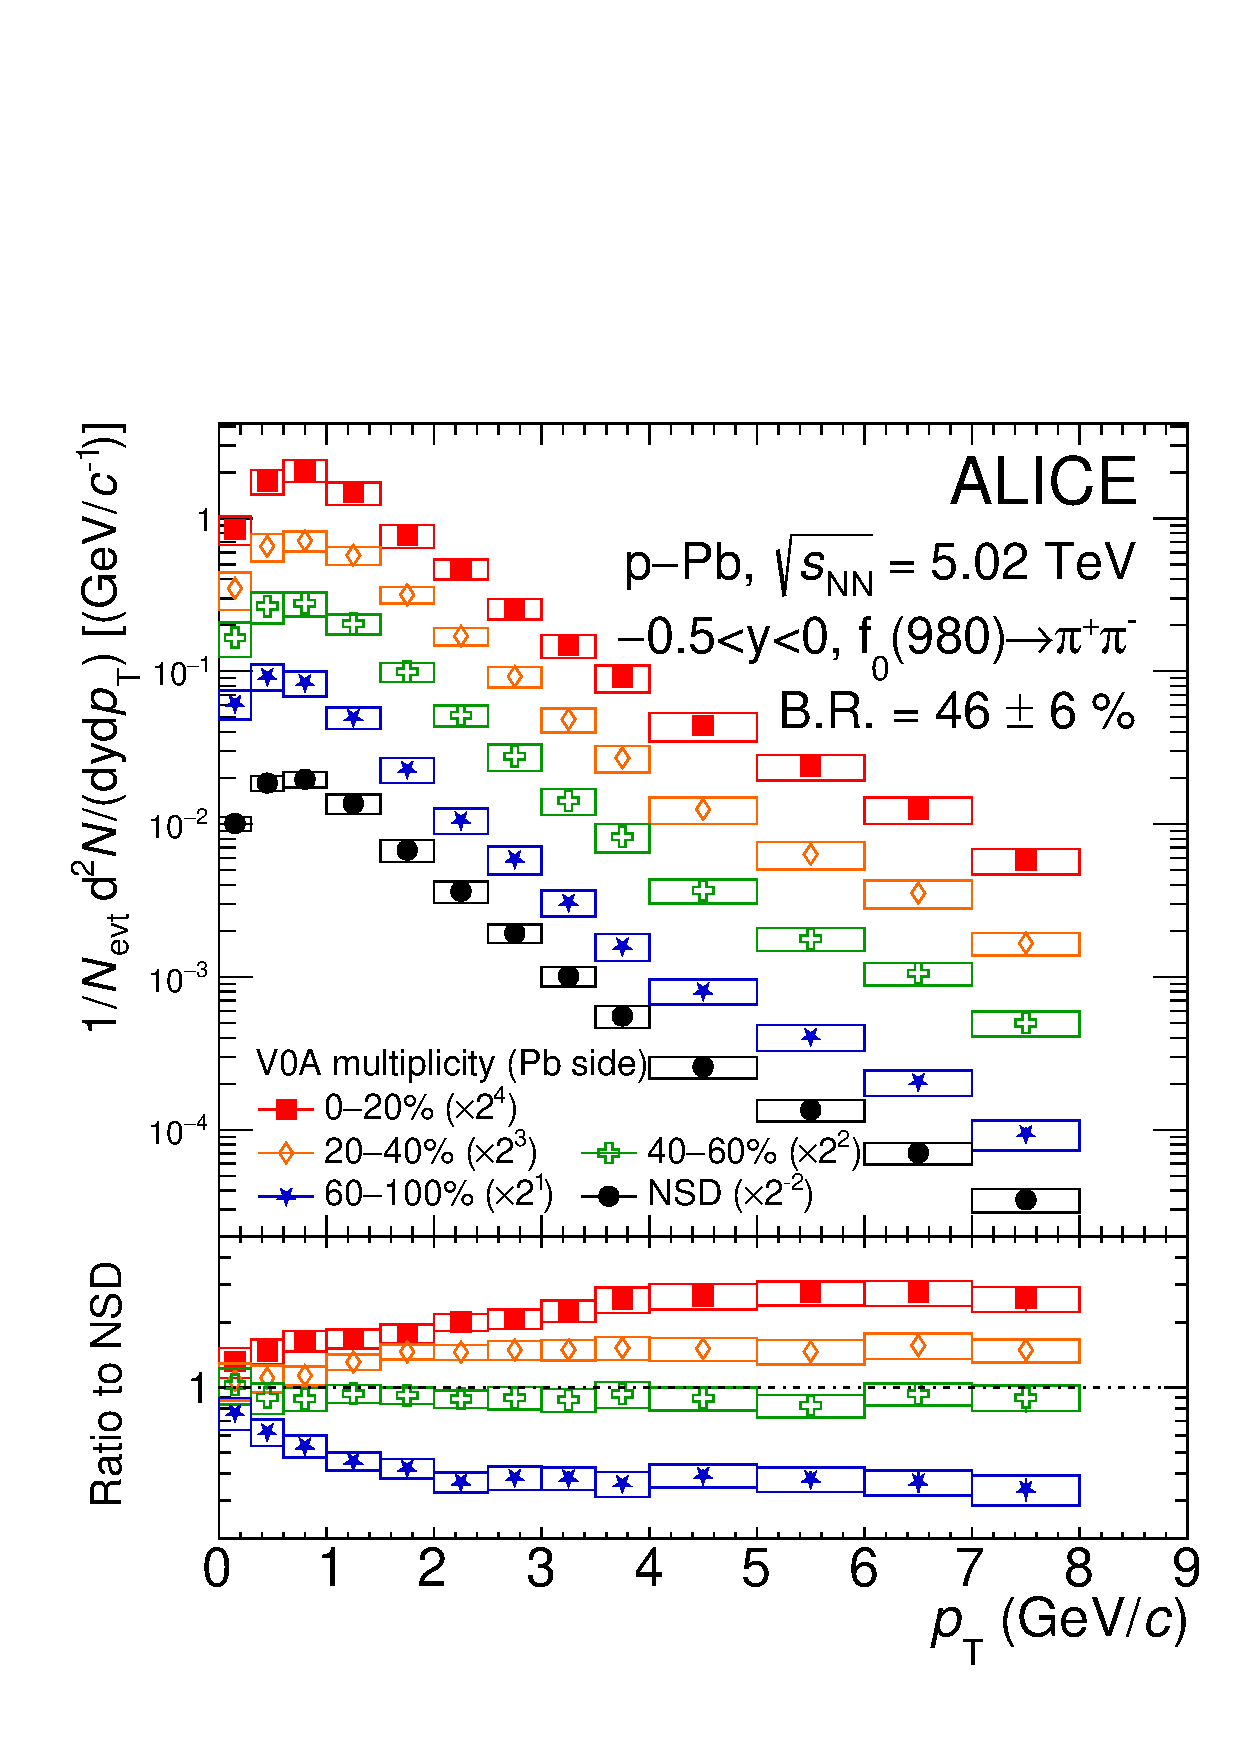
\includegraphics[width=0.6 \textwidth]{figures/Fig2_pt.pdf} }
	\caption{ Transverse momentum spectra of \fzero~in p--Pb collisions at \snn~=~5.02~TeV for different multiplicity classes, which are scaled for visibility. Statistical and systematic uncertainties are shown as error bars and boxes, respectively. The normalization uncertainty of 13\% due to the uncertainty of the $\mathrm{B.R.}$ is not shown in the figure. The lower panel shows the ratios of the spectra in multiplicity classes to the NSD spectrum. }
	\label{fig:pt}
\end{figure}

Figure~\ref{fig:pt} shows the $p_{\mathrm{T}}$ spectra of \fzero~in p--Pb collisions at \snn~=~5.02~TeV measured in the range of 0~$<p_{\mathrm{T}}<$~8~GeV/$c$ for different multiplicity classes and NSD events. The multiplicity classes are defined based on the V0A amplitudes, which are proportional to the multiplicity of particles in the forward rapidity region of the Pb-going side. Each spectrum is scaled by a multiplicative factor denoted in the figure for visibility. The lower panel of Fig.~\ref{fig:pt} shows the ratios of the $p_{\mathrm{T}}$ spectra in different multiplicity classes to the NSD one. The systematic uncertainties of the ratios are estimated by propagating the multiplicity-uncorrelated uncertainties on the individual spectra. For $p_{\mathrm{T}}<$~4~GeV/$c$, a hardening of the $p_{\mathrm{T}}$ spectrum from low- to high-multiplicity events is clearly seen, while the spectral shapes in the different multiplicity classes are found to become consistent among each other for $p_{\mathrm{T}}>$~4~GeV/$c$. Such trends are similar to those observed for other hadronic species~\cite{Schnedermann:1993ws, ALICE:2019hno} and are understood as due to the radial flow.

\begin{table}[h!]
\caption{The values of d$N$/d$y$ and $\left\langle p_{\mathrm{T}} \right\rangle$ for \fzero~measured in p--Pb collisions at \snn~=~5.02~TeV for different multiplicity classes~\cite{ALICE:2012xs}. The first and second uncertainties represent the statistical and systematic uncertainties, respectively}
\centering
\begin{tabular}{ccc}
\hline 
Multiplicity class (V0A) & d$N$/dy & $\left\langle p_{\mathrm{T}} \right\rangle$ (GeV/$c$) \\ \hline
0--20\% & 0.206$\pm$0.005$\pm$0.014 & 1.287$\pm$0.034$\pm$0.010 \\
20--40\% & 0.153$\pm$0.004$\pm$0.010 & 1.250$\pm$0.029$\pm$0.082 \\
40--60\% & 0.113$\pm$0.002$\pm$0.008 & 1.142$\pm$0.025$\pm$0.088 \\
60--100\% & 0.064$\pm$0.001$\pm$0.005 & 0.999$\pm$0.014$\pm$0.080 \\
\hline
\end{tabular}
\label{tab:ymp}
\end{table}

The integrated yield (d$N$/d$y$) and mean $p_{\mathrm{T}}$ $\left( \left\langle p_{\mathrm{T}} \right\rangle \right)$ of \fzero~are calculated by integrating and averaging the $p_{\mathrm{T}}$ spectrum, respectively. Table~\ref{tab:ymp} shows the d$N$/d$y$ and $ \left\langle p_{\mathrm{T}} \right\rangle$ of \fzero~for different multiplicity classes in p--Pb collisions at \snn~=~5.02~TeV. The d$N$/d$y$ of \fzero~is found to increase linearly with charged-particle multiplicity when considering the $\left\langle \mathrm{d}N_{\mathrm{ch}}/\mathrm{d}\eta \right\rangle$ values from Ref.~\cite{ALICE:2012xs}, while the $\left\langle p_{\mathrm{T}} \right\rangle$ exhibits a weak dependence on the charged-particle multiplicity. 

\begin{figure}[!hbt]
	\centering
	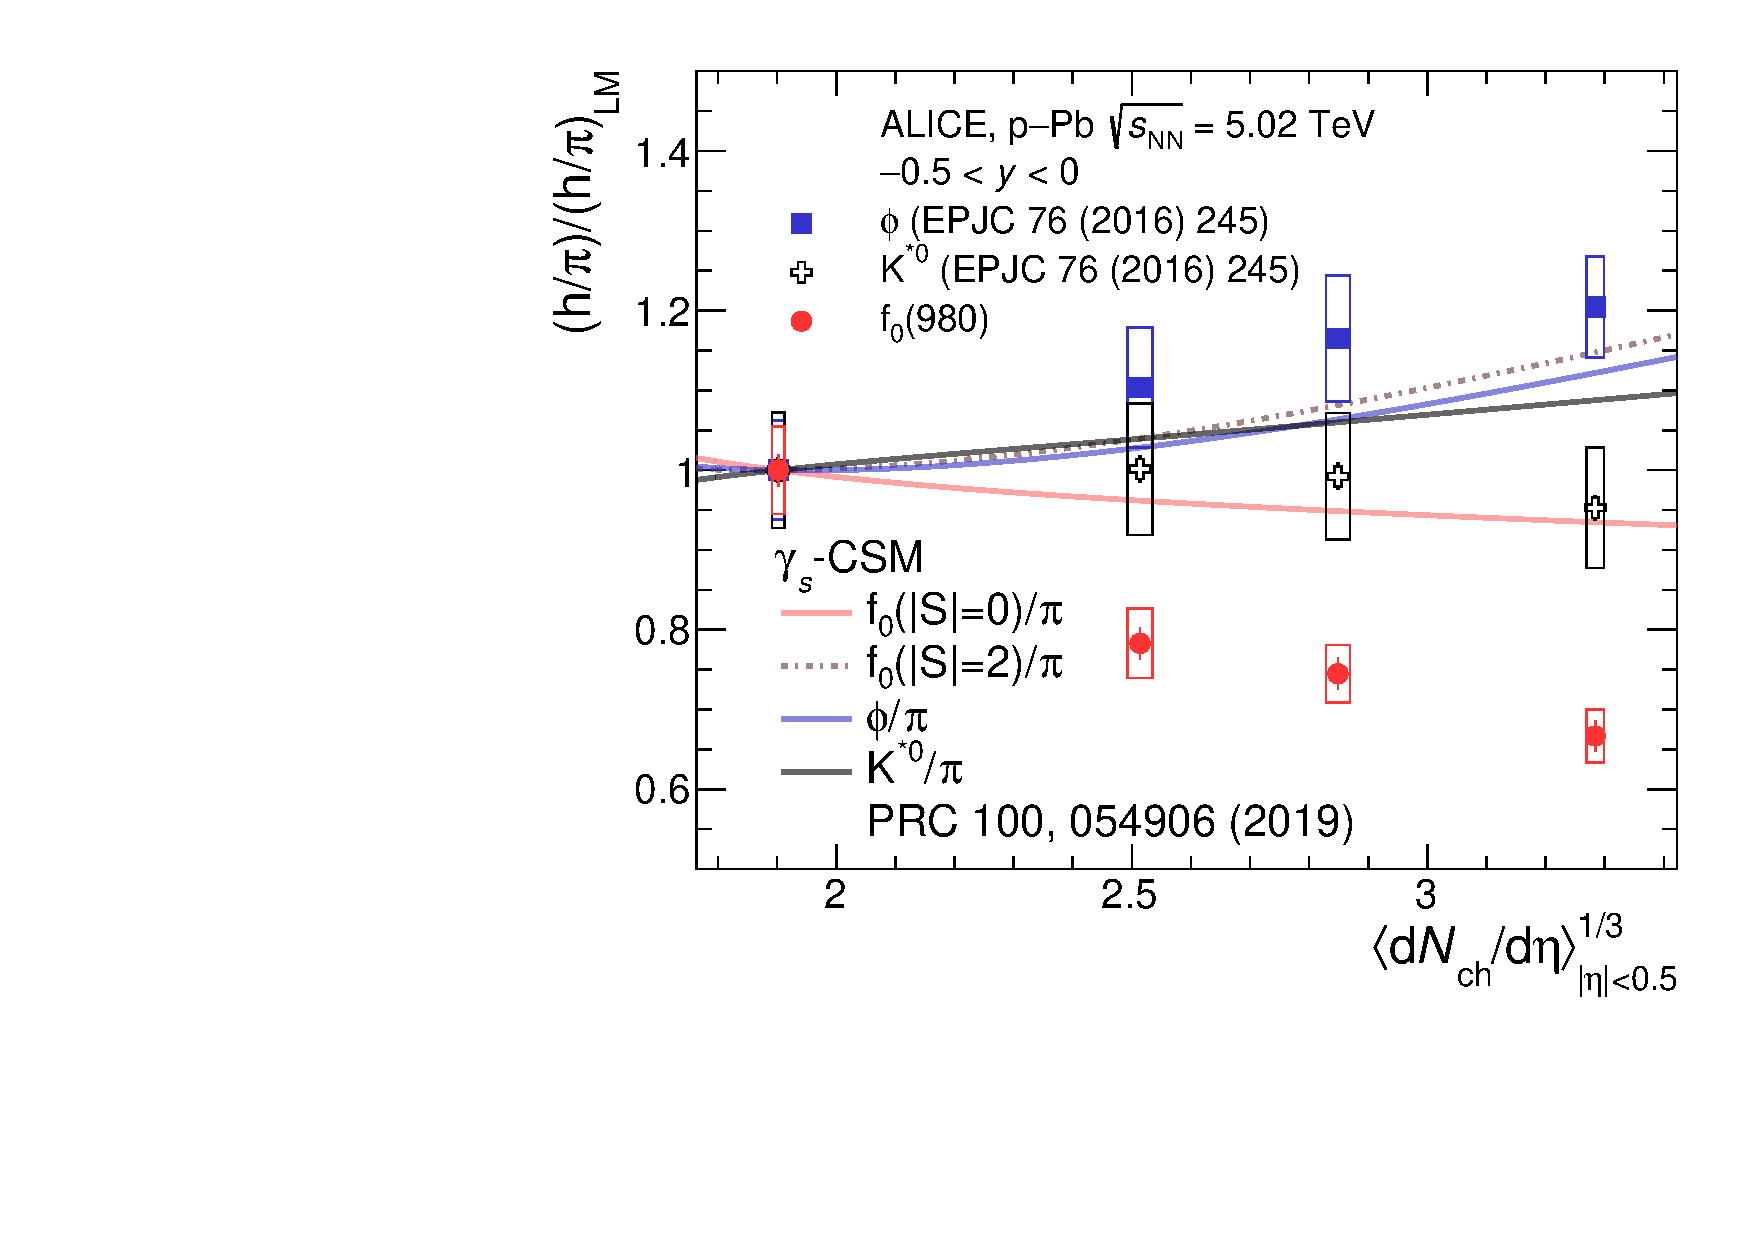
\includegraphics[width=0.49 \textwidth]{figures/Fig4_DR_pion.pdf} 
        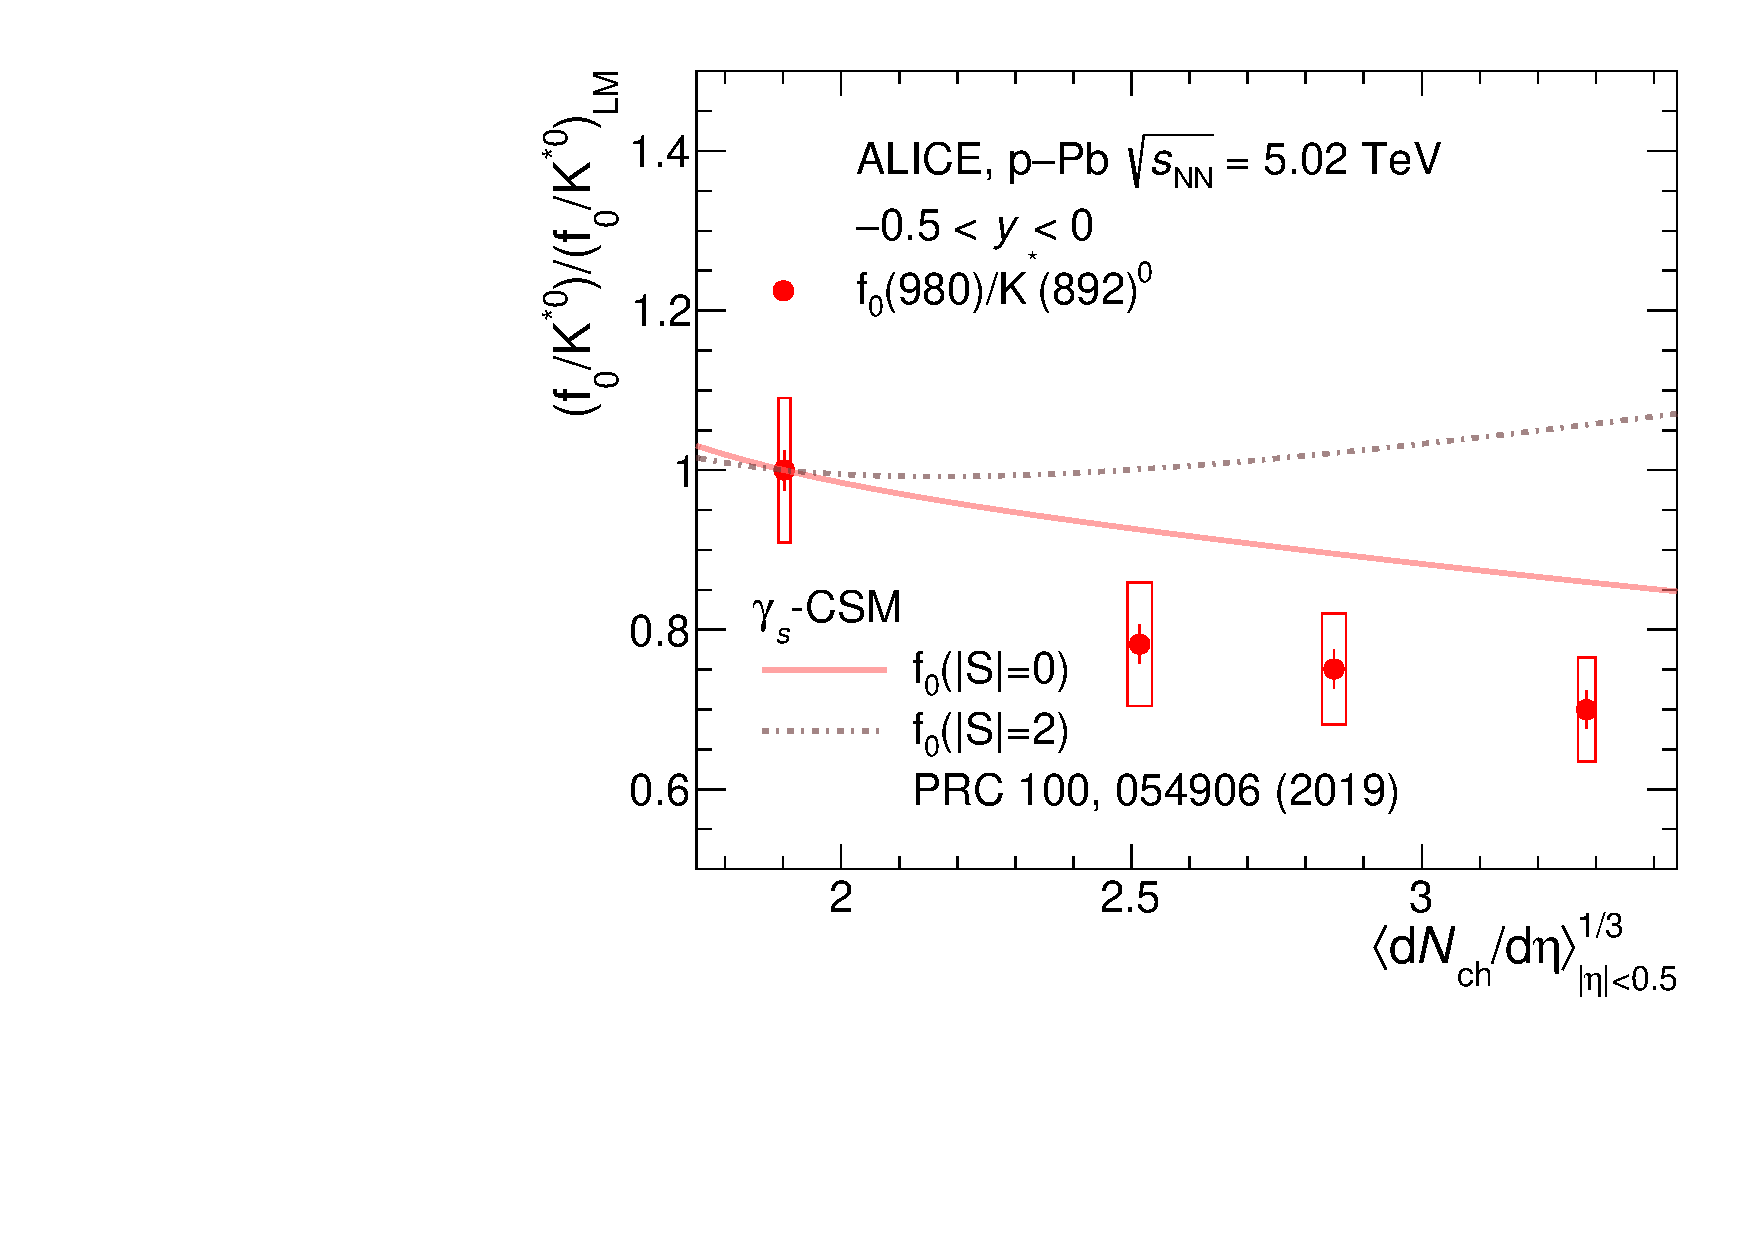
\includegraphics[width=0.49 \textwidth]{figures/Fig5_DR_Kstar.pdf} 
	\caption{ Double ratios of $\phi$~\cite{ALICE:2016sak}, \kstar~\cite{ALICE:2016sak}, and \fzero~to $\pi$~\cite{ALICE:2016dei} (left) and \fzero~to \kstar~(right) as a function of charged-particle multiplicity raised to the power of 1/3. The ratio in each multiplicity class is divided by the ratio in low-multiplicity (LM, 60--100\%) events to allow for a direct comparison among different hadron species and reduce systematic uncertainties. V0A is utilized to categorize events based on their multiplicity. Predictions from the canonical statistical model are represented with lines. }
	\label{fig:f0piAddCSM}
\end{figure}

The multiplicity dependence of \fzero~production is studied by comparing the ratio of the yields of different hadron species to that of pions in different multiplicity classes. A double ratio is calculated by dividing the hadron-to-pion yield ratios to their values measured in the lowest multiplicity interval, $(h/\pi)/(h/\pi)_{\mathrm{LM}}$, allowing a direct comparison of multiplicity dependence among different hadron species and the reduction of the systematic uncertainties. The left panel of Fig.~\ref{fig:f0piAddCSM} shows the double ratios of different particles to charged pion yields as a function of charged-particle multiplicity raised to the power of 1/3 in p--Pb collisions at \snn~=~5.02~TeV. The $\langle \mathrm{d}N/\mathrm{d}\eta \rangle_{|\eta|<0.5}^{1/3}$ is a proxy for the size of the system~\cite{Liu:2018xae}. The systematic uncertainty of the double ratio is calculated considering only the uncorrelated part of the uncertainty. The pion~\cite{ALICE:2016dei}, \kstar~\cite{ALICE:2016sak}, and $\phi$~\cite{ALICE:2016sak} mesons can be classified according to their lifetimes and to their (anti-)strange quark content. The strangeness enhancement and hadronic interactions can be studied by comparing the yield of particles with different characteristics. The double ratio of $\phi$ to $\pi$ increases with increasing multiplicity, which is consistent with the effect of the strangeness enhancement~\cite{ALICE:2016fzo}. Due to the long lifetime ($\approx$~46.2~fm/$c$) of $\phi$ meson, little effect is expected from interactions in the hadronic phase. On the other hand, the double ratio of \kstar~to $\pi$ is independent of multiplicity within the uncertainties even if \kstar~contains one strange quark. The flat trend could be explained by two competing effects, the strangeness enhancement and the interactions of the decay particles in the hadronic medium, due to the short lifetime ($\approx$~4.2~fm/$c$) of \kstar~\cite{ParticleDataGroup:2022pth}. One can expect that hadronic interactions reduce the \kstar~yield if the rescattering dominates over the regeneration. The double ratio of \fzero~to $\pi$ decreases as the multiplicity increases because of the short lifetime ($\approx$~3--5~fm/$c$ from the $\Gamma_{0}^{\mathrm{f}_{0}}$ range estimated from our fits to the \fzero~line shape) of \fzero, suggesting that rescattering effects may play a role. Predictions of the ratio of \fzero~to $\pi$ are shown in Fig.~\ref{fig:f0piAddCSM} (left) for different hidden strangeness assumptions for \fzero~in the $\gamma_{s}$-Canonical Statistical Model (CSM)~\cite{Vovchenko:2019kes}. The CSM considers system-size-dependent hadrochemistry at vanishing baryon density with local conservation of electric charge, baryon density, and strangeness while allowing for undersaturation of strangeness. Note that $\gamma_{s}$ is the parameter for the undersaturation of strangeness and is derived from a fit to the measured particle yields. The CSM hypothesis with two hidden strange quarks predicts an increase of the double ratio, contrary to what is observed experimentally. Moreover, the CSM with zero hidden strangeness predicts the \fzero/$\pi$ ratio to decrease much less than what is measured. When comparing the predicted trend to the measured one, it should however be considered that the CSM does not model interactions in the hadronic phase. The prediction of the CSM for the $\phi/\pi$ ratio qualitatively reproduces the increasing trend of the data with increasing multiplicity, where the hidden strangeness of $\phi$ is two. However, the CSM overestimates the ratio of \kstar~to $\pi$ at high multiplicity because the modification of \kstar~yields due to rescattering effects is not implemented in the CSM, while the strangeness enhancement for \kstar~is regarded.

The right panel of Fig.~\ref{fig:f0piAddCSM} shows the double ratio of the \fzero~to \kstar~yield as a function of $\left\langle \mathrm{d}N_{\mathrm{ch}}/\mathrm{d}\eta \right\rangle^{1/3}$ together with the predictions from the CSM with different hidden strangeness assumptions. The lifetimes of \fzero~and \kstar~are estimated to be of similar order of magnitude and both smaller than the duration of the hadronic phase in p--Pb collisions~\cite{ParticleDataGroup:2022pth}. This leads to the expectation that the \fzero/\kstar~ratio is weakly affected by hadronic interactions, which depend on the hadronic cross section of the different decay products of the two resonances. The measured double ratio shows a decreasing trend with increasing multiplicity, which is qualitatively described with the zero-hidden-strangeness assumption for \fzero~and can be explained by the strangeness enhancement of the \kstar~yield. The CSM prediction with the assumption of two hidden strange quarks is mildly increasing as the multiplicity increases, a trend that is opposite to the experimental result. The differences between the data point at the highest multiplicity and the two predictions with zero and two strange quarks amount to 2.3 and 5.2 standard deviations, calculated using the total uncertainty on the measurement, respectively. Therefore, the decreasing trend of the double ratio of \fzero~to \kstar~can suggest no effective strangeness enhancement for the \fzero. The discrepancies between the data and the model predictions can be attributed to the assumption of the same modification of \fzero~and \kstar~yields from hadronic interactions while the decay products from \fzero~and \kstar~differ.

\begin{figure}[!hbt]
	\centering
	\subfigure{ 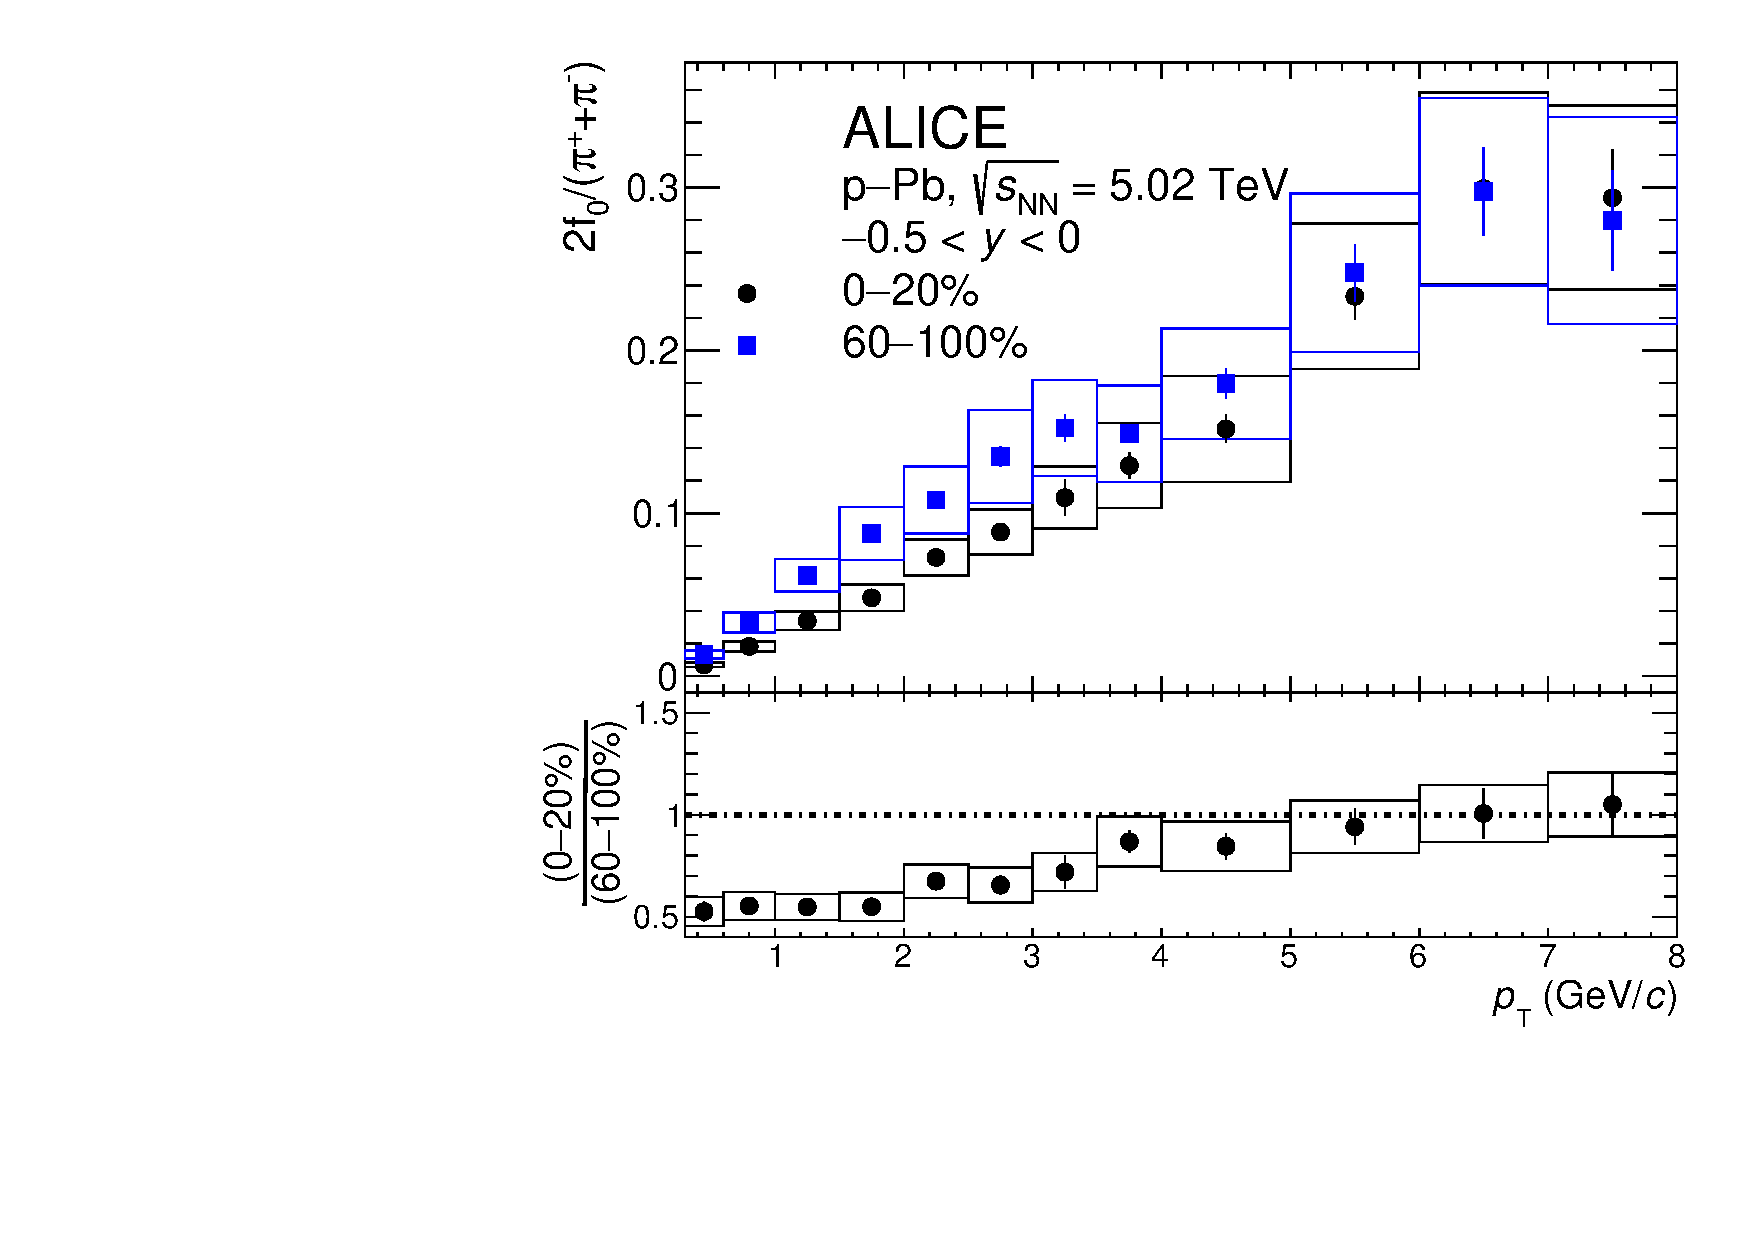
\includegraphics[width=0.6 \textwidth]{figures/Fig6_DR_pt_pion.pdf} }
	\caption{ The particle yield ratios of \fzero~to $\pi$ as a function of $p_{\rm{T}}$ in high-multiplicity (circles) and low-multiplicity (squares) p--Pb collisions at \snn~=~5.02~TeV. The lower panel shows the double ratio of \fzero/$\pi$ between the high-multiplicity and low-multiplicity events. V0A is utilized to categorize events based on their multiplicity.}
	\label{fig:f0piPt}
\end{figure}

Figure~\ref{fig:f0piPt} shows the $p_{\mathrm{T}}$-differential particle yield ratio of \fzero~to $\pi$ in high-multiplicity (HM, 0--20\%) and low-multiplicity (LM, 60--100\%) p--Pb collisions at \snn~=~5.02~TeV. The ratios are consistent with each other within one sigma at $p_{\mathrm{T}}>$~4~GeV/$c$, while at lower $p_{\mathrm{T}}$ the \fzero~to $\pi$ ratio is systematically lower in the HM class as compared to the LM one. This suppression of \fzero~production at high multiplicity and low $p_{\mathrm{T}}$ is quantified via the double ratio reported in the lower panel of Fig.~\ref{fig:f0piPt}. In the double ratio, the correlated uncertainties across multiplicity classes cancel. The $p_{\mathrm{T}}$ dependence of the double ratio indicates that the suppression of the $p_{\mathrm{T}}$-integrated yield shown in Fig.~\ref{fig:f0piAddCSM} is mainly occurring at low $p_{\mathrm{T}}$ values ($p_{\mathrm{T}}<$~3.5~GeV/$c$), showing a qualitatively similar $p_{\mathrm{T}}$ dependence as the one reported in Ref.~\cite{ALICE:2019etb} for the suppression of the \kstar$\rm{}/K$ ratios.

\begin{figure}[!hbt]
	\centering
	\subfigure{ 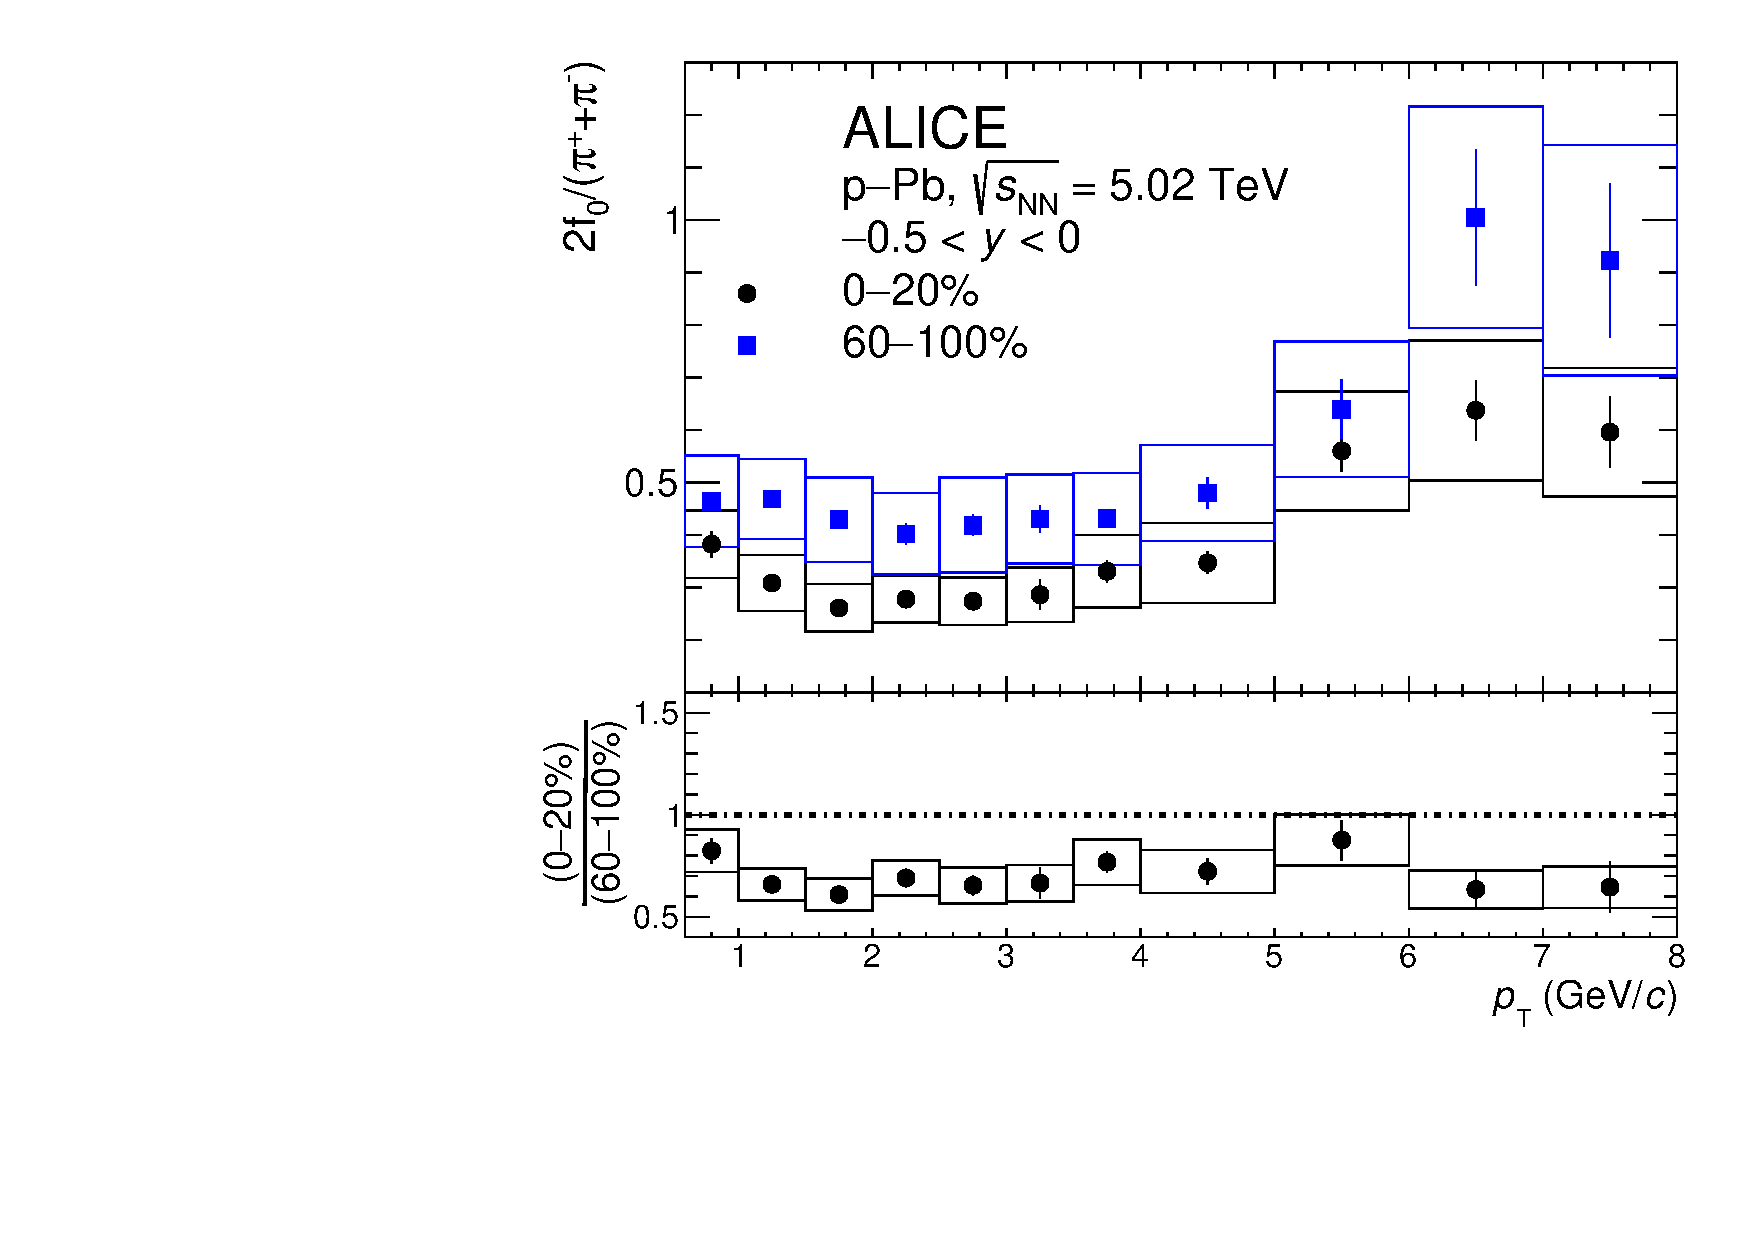
\includegraphics[width=0.6 \textwidth]{figures/Fig6_DR_pt_kstar.pdf} }
	\caption{The particle yield ratio of \fzero~to \kstar~as a function of $p_{\rm{T}}$ in high-multiplicity (circles) and low-multiplicity (squares) p--Pb collisions at \snn~=~5.02~TeV. The lower panel shows the double ratio of high-multiplicity to low-multiplicity \fzero/\kstar. V0A is utilized to categorize events based on their multiplicity. }
	\label{fig:f0KsPt}
\end{figure}

Figure~\ref{fig:f0KsPt} shows the $p_{\mathrm{T}}$-differential particle yield ratio of \fzero~to \kstar~in HM and LM p--Pb collisions at \snn~=~5.02~TeV. The ratio in HM events is lower than that in LM events in the entire $p_{\mathrm{T}}$ range, in contrast to what is observed for \kstar$\rm{}/K$ and \fzero/$\pi$ ratios for which the suppression is observed only at low $p_{\mathrm{T}}$. The suppression of the \fzero/\kstar~ratio in HM events for $p_{\mathrm{T}}>$~4~GeV/$c$ is evaluated to be 0.70~$\pm$~0.04 (stat) $\pm$~0.05 (syst) by fitting the double ratio with a constant function and indicates that other effects, beyond hadronic interactions, are present. For instance, the strangeness enhancement can explain the suppression of the \fzero~yield relative to that of \kstar~under the assumption that the \fzero~does not have strange quark content. This argument is also consistent with the decreasing trend of the $p_{\mathrm{T}}$-integrated \fzero/\kstar~ratio with increasing multiplicity and their comparison to the CSM calculations shown in Fig.~\ref{fig:f0piAddCSM}. In summary, the suppression of the \fzero/\kstar~ratio may suggest that the \fzero~does not contain strange quarks, and its production is therefore not affected by the strangeness enhancement. In addition, the enhancement of baryon-to-meson ratio at intermediate $p_{\mathrm{T}}$, observed for p/$\phi$, $\Lambda$/$\mathrm{K}_{\mathrm{s}}^{0}$, $\Xi$/$\phi$, and $\Omega$/$\phi$ ratios~\cite{ALICE:2020jsh}, is not seen in the \fzero/\kstar~ratio, providing a hint that the number of constituent quarks for \fzero~is two.

\begin{figure}[!hbt]
	\centering
	\subfigure{ 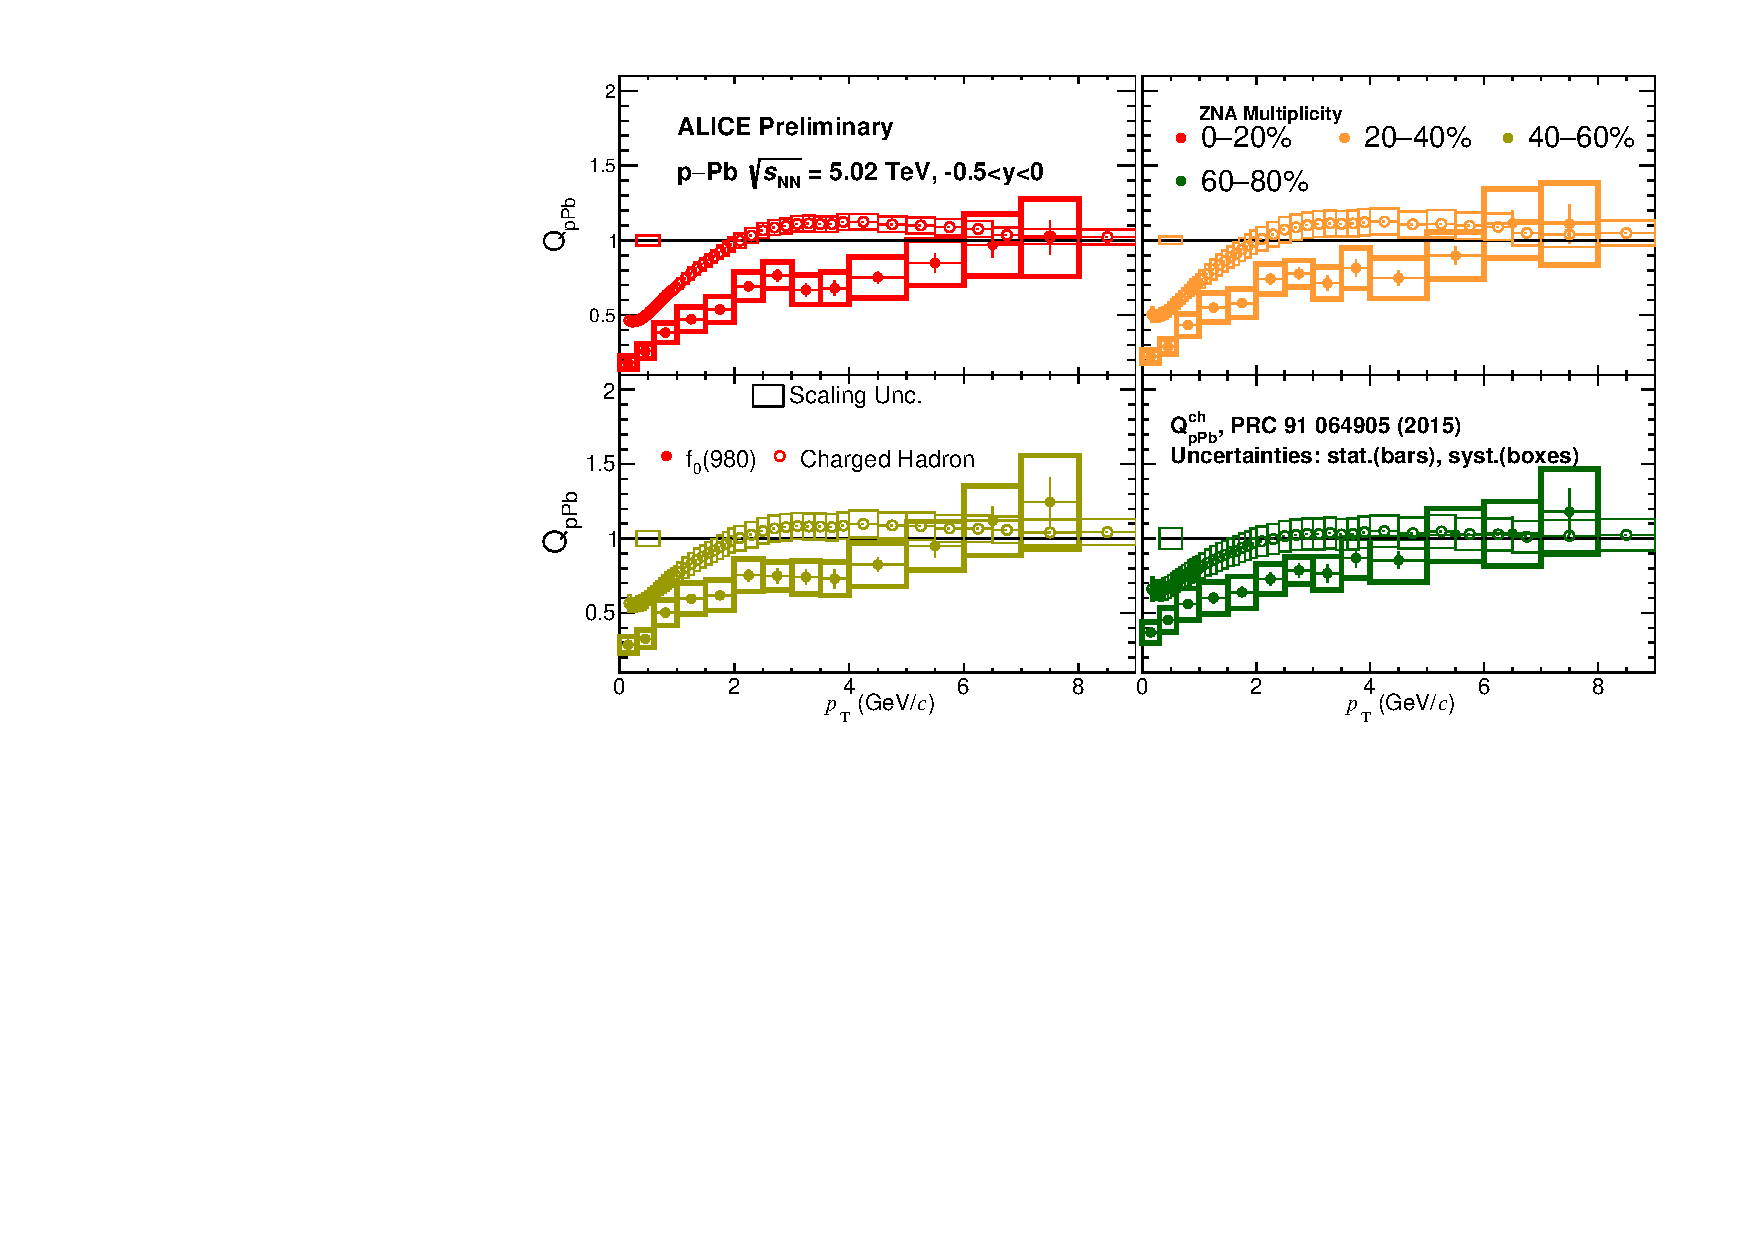
\includegraphics[width=0.8 \textwidth]{figures/Fig7_QpPb.pdf} }
	\caption{ Nuclear modification factor ($Q_{\rm{pPb}}$) of \fzero~as a function of $p_{\rm{T}}$ in p--Pb collisions at \snn~=~5.02~TeV for different multiplicity classes. The multiplicity class is defined with the ZNA, which is the ZN placed on the Pb-going side. Statistical and systematic uncertainties are shown as error bars and boxes, respectively. Black boxes around unity represent the binary collision scaling uncertainties. The $Q_{\rm{pPb}}$ of charged hadrons~\cite{ALICE:2014xsp} are reported for comparison. }
	\label{fig:QpPb}
\end{figure}

The $p_{\rm{T}}$-differential yield of \fzero~in p--Pb collisions can be compared to the one in pp collisions at the same center-of-mass energy by computing the nuclear modification factor $Q_{\mbox{pPb}}$, defined as 
\begin{eqnarray}
Q_{\mbox{pPb}} = \dfrac{\mathrm{d}^{2} N_{\mathrm{f}_{0}(980)}^{\mathrm{pPb}} / \mathrm{d} p_{\mathrm{T}} \mathrm{d}y }{ \left\langle T_{\mathrm{pPb}} \right\rangle \mathrm{d}^{2} \sigma_{\mathrm{f}_{0}(980)}^{\mathrm{pp}}/ \mathrm{d} p_{\mathrm{T}} \mathrm{d}y },
\end{eqnarray}
where $\left\langle T_{\mathrm{pPb}} \right\rangle$ is the average nuclear overlap function, which is proportional to the number of binary nucleon--nucleon collisions, for the considered centrality class, and $\mathrm{d}^{2} \sigma_{\mathrm{f}_{0}(980)}^{\mathrm{pp}}/ \mathrm{d} p_{\mathrm{T}} \mathrm{d}y$ is the $p_{\mathrm{T}}$ differential cross-section for \fzero~production in pp collisions taken from Ref.~\cite{ALICE:2022qnb}. For this study, the centrality classes are defined using an event selection based on the ZN calorimeter in the Pb-going direction (ZNA) to minimize the possible selection biases, as reported in Ref~\cite{ALICE:2014xsp}.

Figure~\ref{fig:QpPb} shows the $Q_{\mbox{pPb}}$ of \fzero~in p--Pb collisions at \snn~=~5.02~TeV in different multiplicity classes. The systematic uncertainties are calculated with the assumption that there is no correlated uncertainty between the yield in pp and p--Pb collisions except for the B.R. uncertainty, which cancels out in the ratio. The scaling uncertainty on the $Q_{\mbox{pPb}}$ shown in Fig.~\ref{fig:QpPb} is due to the uncertainty on $\left\langle T_{\mathrm{pPb}} \right\rangle$, which is taken from Ref.~\cite{ALICE:2014xsp}. The $Q_{\mbox{pPb}}$ distributions of \fzero~are compared to those of charged hadrons~\cite{ALICE:2014xsp}. At low $p_{\mathrm{T}}$ ($p_{\mathrm{T}}<$~4~GeV/$c$), the $Q_{\mbox{pPb}}$ of \fzero~is lower than unity indicating a suppression of the production in p--Pb collisions relative to pp collisions. This suppression becomes more pronounced with increasing multiplicity. Moreover, for $p_{\mathrm{T}}<$~4~GeV/$c$ the $Q_{\mbox{pPb}}$ of \fzero~is also lower than that of charged hadrons and the difference increases with increasing multiplicity. As $p_{\mathrm{T}}$ increases, \fzero~$Q_{\mbox{pPb}}$ values become compatible with those for charged particles, reaching unity. The dependencies of the nuclear modification factor on the multiplicity and $p_{\mathrm{T}}$ clearly indicate that rescattering largely contributes to the strong suppression of the \fzero~yield for $p_{\mathrm{T}}<$~4~GeV/$c$. In addition, the $Q_{\mbox{pPb}}$ does not exhibit a significant Cronin-like enhancement~\cite{Cronin:1974zm} at intermediate $p_{\mathrm{T}}$ in HM events. Since baryons show a more pronounced Cronin peak as compared to conventional mesons~\cite{ALICE:2016dei, ALICE:2021rpa}, the absence of a significant Cronin-like enhancement of \fzero~might suggest that the \fzero~is composed of two quarks.